\documentclass[a4paper,11pt]{article}
\usepackage[margin=2cm]{geometry}
%\usepackage[utf8]{inputenc}
\usepackage{amsmath}
\usepackage{float}
\usepackage{stanli}
\usepackage{tikz}
\usetikzlibrary{arrows.meta,arrows,positioning}
\usepackage{ifthen}
\usepackage{adjustbox}
\usepackage[gobble=auto]{pythontex}
\usepackage[nameinlink]{cleveref}
\usepackage{graphicx}
\usepackage[absolute,overlay]{textpos}
\graphicspath{ {./images/CIV5121/} }
% Differential
\newcommand*{\D}{\mathrm{d}}
% scientific notation
\providecommand{\e}[1]{\ensuremath{\times~10^{#1}}} 

\begin{pycode}
	import math
	def n(num, sig=3):
		f = '%.' + str(sig) + 'g' 
		ret = f % num
		if 'e' in ret:
			ret = ret.replace('e', r'\e{')
			ret += '}'
		return ret
	
	def to_eng(num, sig=3):
		try:
			x = int(math.log10(num)//3)*3
		except (ValueError, KeyError):
			x = 0
		if x != 0:
			ret = str(n(num/10**x,sig)) + r' \times 10^{' + str(x) + '}'
		else:
			ret = str(n(num,sig))
		return ret
\end{pycode}

% Commands for jinja2 templating
% Instead of empty braces (i.e. no command effect), here we make the variable uppercase red
% to emphasize in the template those variables to be replaced. Once rendered, this formatting
% has not effect as jinja replaces the \VAR{variable} entirely.
\usepackage{xcolor}
\newcommand*{\VAR}[1]{\textcolor{red}{\textbf{#1}}}
\newcommand*{\BLOCK}[1]{\textcolor{red}{\textbf{#1}}}

\usepackage{comment}
\newif\ifhidden
% This defines whether to show the hidden content or not.
\hiddenfalse 
\ifhidden 	% if \ hiddentrue
	\excludecomment{hidden}	% Exclude text within the "hidden" environment
\else   	% \ hiddenfalse
	\includecomment{hidden}		% Include text in the "hidden" environment
\fi

\title{Final assessment: CIV5121 Building structures and technology (Clayton)\\
\VAR{FullName} (\VAR{StudentID})}
\date{Semester 2, 2020}
\usepackage{times}
\begin{document}
\maketitle
%\thispagestyle{fancy}

\begin{introduction}	
\noindent
\textbf{Introduction}\\
\noindent
This exam is an open-book assessment. The answers provided to all questions must be submitted through Moodle. You are allowed to use computational aid (including calculators), and to refer to lecture notes or other materials (that must be properly cited and referenced in order to avoid plagiarism).\\
\\ 
\noindent
Exam duration: 2 hours and 10 mins\\
\noindent
Scanning time: 30 mins\\

\end{introduction}
\begin{textblock*}{5cm}(8.9cm,28.49cm)
Page
\end{textblock*}
\begin{textblock*}{5cm}(10.1cm,28.49cm)
of 5
\end{textblock*}
%{\sf\tighttoc}
\newpage
\noindent
\textbf{QUESTION 1 [5 marks]}\\
Explain the key features of cavity wall construction\\
\\
\\
\begin{pycode}
	from testscript import *
	import random
	import math
	fn = open('read2.txt','r')
	for content in fn:
		iterator = int(content)
	fn.close()
	
	def allocation(aa, b):
		length = len(aa)
		product = []
		result = []
		fullproduct = 1
		for obj in aa:
			fullproduct = fullproduct * obj
		for i in range(1, length):
			product.append(1)
			for i in range(i, length):
				product[-1] = product[-1] * aa[i]
		r1= b%fullproduct
		for i in range(1, length):
			d1 = int(r1/product[i - 1])
			r1 = r1%product[i - 1]
			result.append(d1)
		result.append(r1)
		return result
	
	# ============================= Question 2 ============================
	para2_1 = [4, 3]
	para2_2 = [3, 3, 3]
	al2_1 = allocation(para2_1, iterator)
	al2_2 = allocation(para2_2, iterator)
		
	select21 = al2_1[0]
	select22 = al2_1[1]
	select23 = al2_2[0]
	select24 = al2_2[1]
	select25 = al2_2[2]
	v21 = [2.8, 3, 3.2, 3.4]
	v22 = [3.5, 4.5, 5]
	v23 = [1.5, 2.5, 3.5]
	v24 = [20, 30, 40]
	v25 = [0.5, 0.8, 1.1]
	
	sv21 = v21[select21]
	sv22 = v22[select22]
	sv23 = v23[select23]
	sv24 = v24[select24]
	sv25 = v25[select25]
	
	# ============================= Question 3 ============================
	para3_1 = [4, 4]
	para3_2 = [4]
	al3_1 = allocation(para3_1, iterator)
	v31 = [3, 3.5, 4, 4.5]
	v32 = [0.5, 1, 1.5, 2]
	v33 = [7800, 8000, 8200, 8400]
	
	sv31 = v31[al3_1[0]]
	sv32 = v32[al3_1[1]]
	sv33 = v33[iterator%4]
	
	# ============================= Question 4 ============================
	v41 = [400, 450, 500]
	v42 = [350, 400, 450]
	v43 = [1500, 1700, 1900, 2100]
	v44 = [1500, 1700, 1900, 2100]
	
	sv41 = v41[iterator%3]
	sv42 = v42[iterator%3]
	sv43 = v43[iterator%4]
	sv44 = v44[iterator%4]
	
	# ============================= Question 5 ============================
	para5_1 = [5, 4, 4]
	al5_1 = allocation(para5_1, iterator)
	para5_2 = [2, 2, 2, 2]
	al5_2 = allocation(para5_2, iterator)
	v51 = [3, 3.2, 3.4, 3.6, 4]
	v52 = [6, 6.2, 6.4, 6.6]
	v53 = [280, 300, 320, 350]
	v54 = [60, 80]
	v55 = [0.8, 0.9]
	v56 = [150, 200]
	v57 = [0.8, 0.9]
	
	sv51 = v51[al5_1[0]]
	sv52 = v52[al5_1[1]]
	sv53 = v53[al5_1[2]]
	sv54 = v54[al5_2[0]]
	sv55 = v55[al5_2[1]]
	sv56 = v56[al5_2[2]]
	sv57 = v57[al5_2[3]]
	
	L_list = [3.5,3.75,4.0,4.25,4.5,4.75,5.0]  # m
	M_list = [-80, -30, -50]	# kNm
	I = 37.5e-6 	# m4
	J = 75e-6   	# m4
	E = 200     	# GPa
	G = 80      	# GPa
	
	# Unit conversions MNm2
	E *= 1e3
	G *= 1e3
	
	L = random.choice(L_list) 		# Member length
	M = random.choice(M_list) 		# y-axis moment load @ C
	
	grid = [L,I,J,E,G,M]
	
	EI_L = E*I/L
	GJ_L = G*J/L
	
	# Call analysis
	D = solve_D(grid)
	theta_C, theta_D, theta_F = D
	Fcd = eleF(eleK(grid),d_CD(D)*1e3)
	Fce = eleF(eleK(grid),d_CE(D)*1e3)
	Fcf = eleF(eleK(grid),d_CF(D)*1e3)
	Fgc = eleF(eleK(grid),d_GC(D)*1e3)
	Fcg = eleF(eleK(grid),d_CG(D)*1e3)
	
	bmd_scale=8
	tmd_scale=5
	
	iterator = iterator + 1
	fn = open('read2.txt','w')
	fn.write('%d' % iterator)
	fn.close()
\end{pycode}
\noindent
\textbf{QUESTION 2 [20 marks]}\\
One span of a simply supported composite slab using Condeck HP metal sheeting 0.75 mm in a composite floor structure of an office building is given in Figure 1 with an overall thickness of 130 mm. The span length L is $\py{sv21}$ m. The live load is $\py{sv22}$ kPa. The dead load consists of the floor self-weight plus a super-imposed dead load of $\py{sv23}$ kPa. There is a point load P of $\py{sv24}$ kN per meter width because of partition wall at a distance \emph{a} of $\py{sv25}$ m from the left end support.\\
\\
Take f'\textsubscript{c} = 32 MPa, E\textsubscript{c}=28000 MPa and unit weight of reinforced concrete = 25 kN/m\textsuperscript{3}.
\\
a) Check if the ultimate bending capacity is sufficient or not for the mid-span section. \textbf{[10 marks]}
\\
b) Check if the ultimate bending capacity is sufficient or not for the section with the point load P (see Figure 1 below). \textbf{[10 marks]}
\begin{figure}[ht]
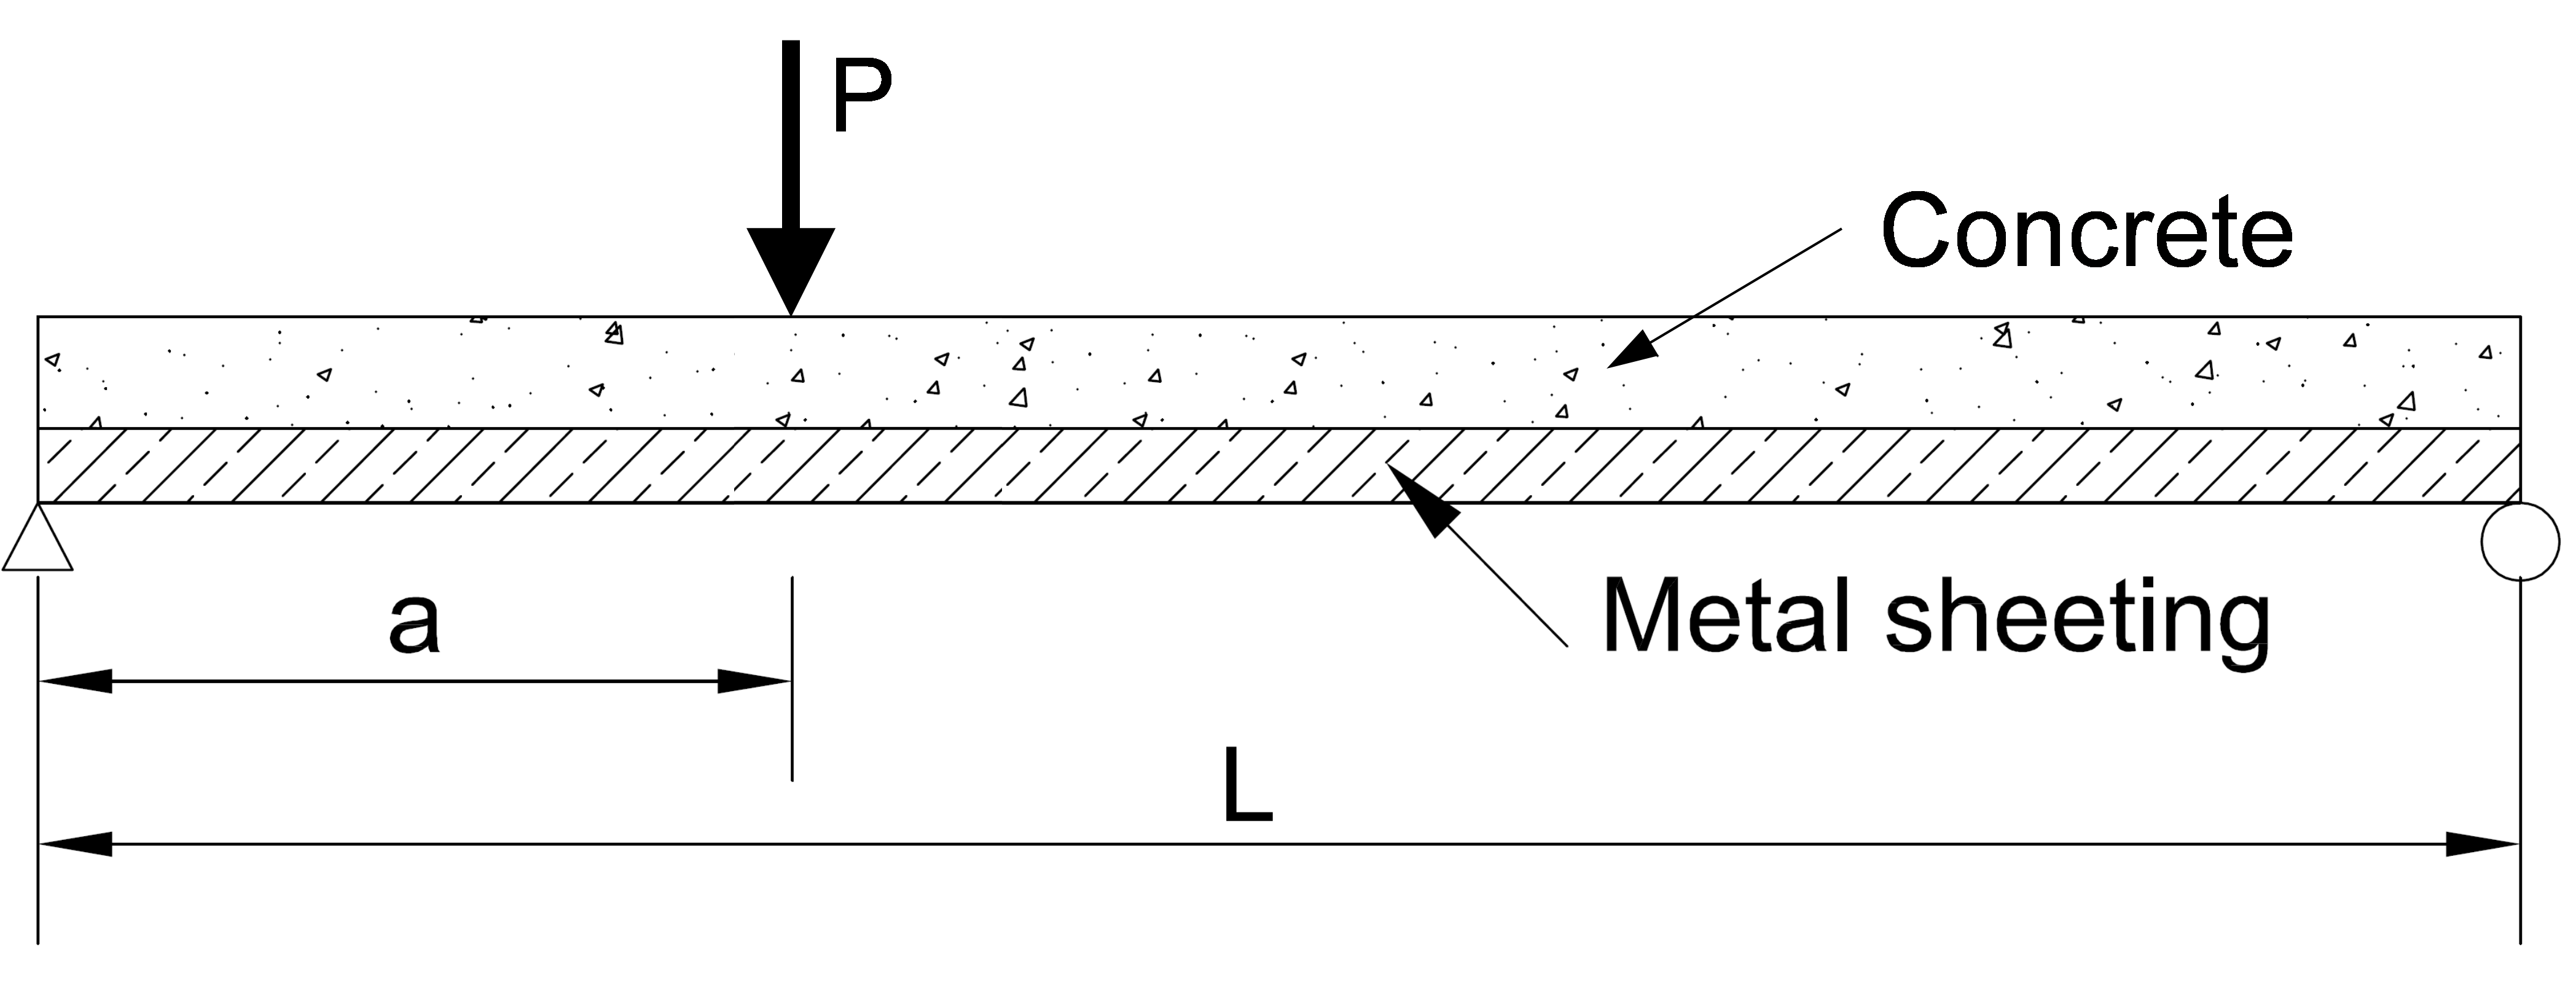
\includegraphics[width=8cm, height=3.05cm]{Figure1.png}\\
\centering
Figure 1\\
\centering
\end{figure}
\\
\noindent
\textbf{QUESTION 3 [20 marks]}\\
The layout and cross section of a composite floor structure (composite slab and secondary composite beams) in a building is shown in Figure 2 below. All secondary beams are simply supported. The live load is $\py{sv31}$ kPa. The dead load consists of the floor self-weight plus $\py{sv32}$ kPa super-imposed dead load. Take f'\textsubscript{c} = 32 MPa, E\textsubscript{c} = 28000 MPa, the height of metal sheeting rib h\textsubscript{r} = 55 mm, unit weight of reinforced concrete = 25 kN/m\textsuperscript{3}.
\\
\\
a) What is the maximum span length that the secondary composite beam (see Section a-a) could achieve based on its positive moment capacity and the applied dead and live loads given above. take the effective width of the composite beam b\textsubscript{cf} = 1100 mm. \textbf{[10 marks]}\\
\\
b) If the span length L = $\py{sv33}$  mm, and the shear studs (d\textsubscript{bs} = 19 mm, f\textsubscript{uc} = 410 MPa) are placed at one row with a spacing of 200 mm, please calculate the positive moment capacity of the secondary composite beam. \textbf{[10 marks]}\\
\begin{textblock*}{5cm}(8.9cm,28.49cm)
Page
\end{textblock*}
\begin{textblock*}{5cm}(10.1cm,28.49cm)
of 5
\end{textblock*}
\newpage
\noindent
\begin{figure}[ht]
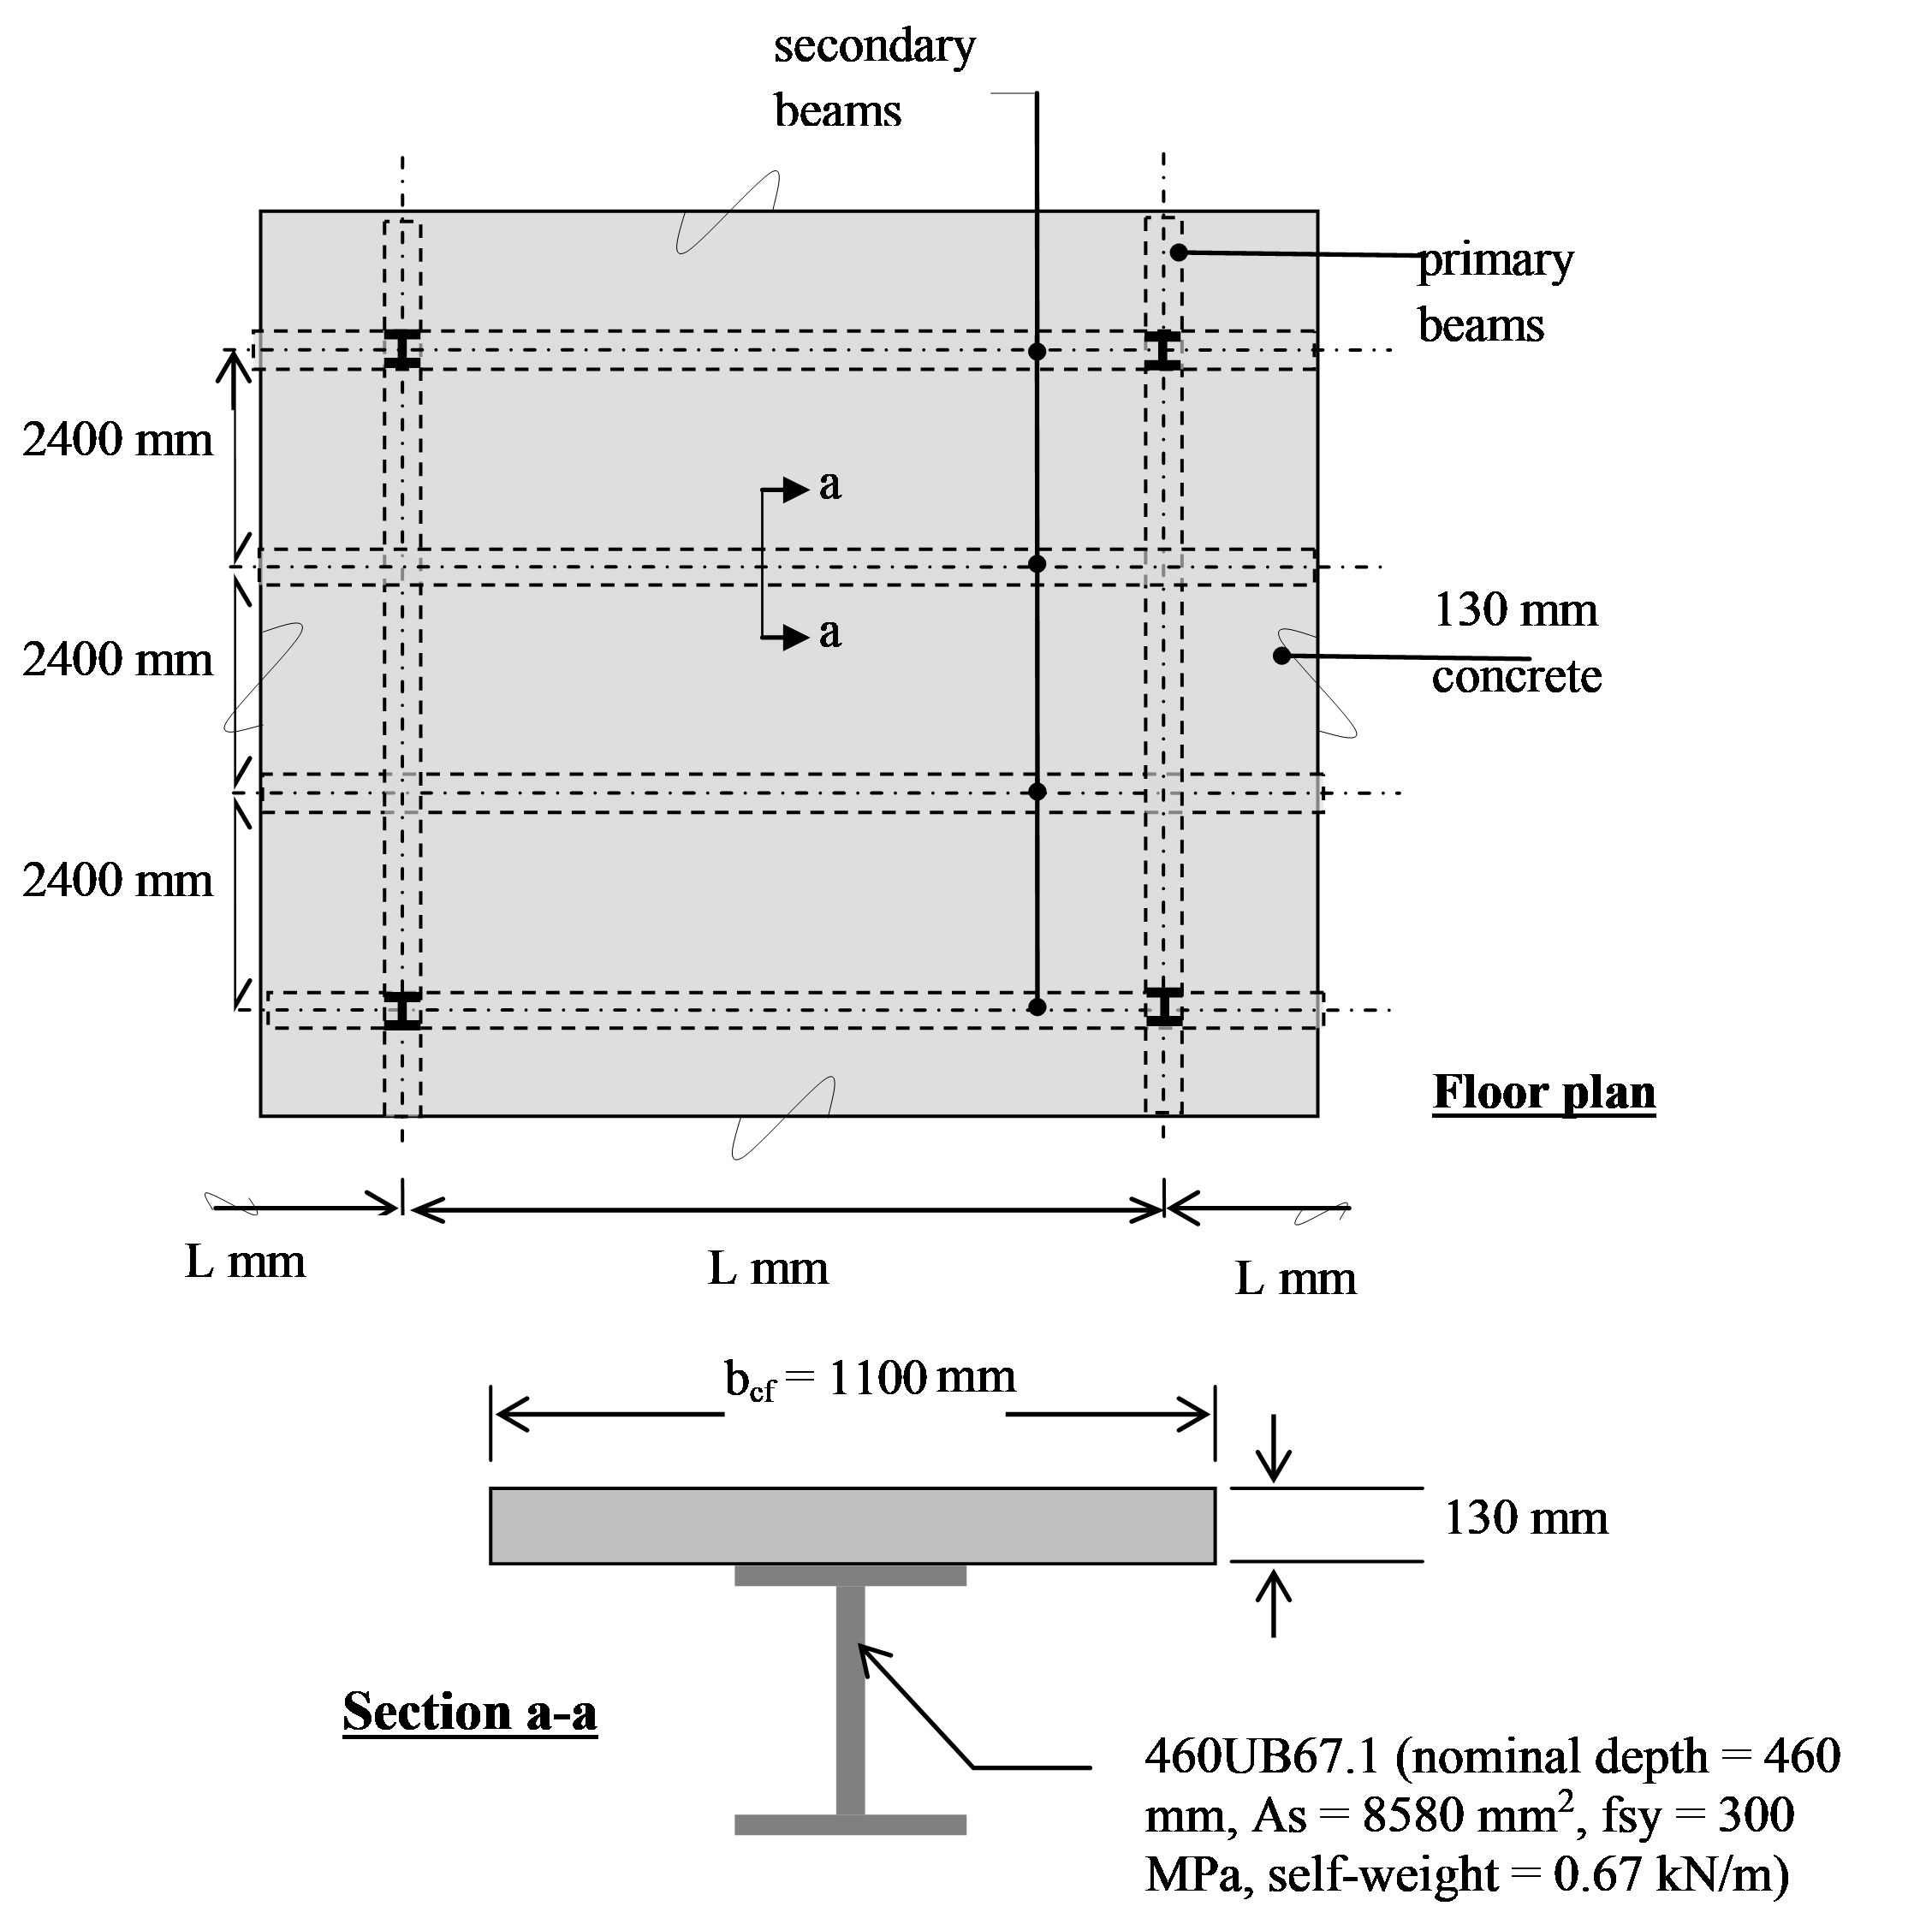
\includegraphics[width=15.92cm, height=15.81cm]{Figure2.png}\\
\centering
Figure 2\\
\centering
\end{figure}
\\
\begin{textblock*}{5cm}(8.9cm,28.49cm)
Page
\end{textblock*}
\begin{textblock*}{5cm}(10.1cm,28.49cm)
of 5
\end{textblock*}
\newpage
\noindent
\textbf{QUESTION 4 [10 marks]}\\
Assuming that a typical column rests on a rectangular footing through a X\textsubscript{c}$\times$Y\textsubscript{c} ($\py{sv41}$$\times$$\py{sv42}$) mm base plate, calculate the maximum design column load N* the footing can support in terms of punching shear. Assume planar dimensions of the footing to be X\textsubscript{b}$\times$Y\textsubscript{b} ($\py{sv43}$$\times$$\py{sv44}$) mm and its overall depth D = 500 mm with a cover concrete thickness of 75 mm. The concrete compressive strength f'\textsubscript{c} is 32 MPa and the steel reinforcements (f\textsubscript{y}=500 MPa) are placed as shown in Figure 3.\\
\begin{figure}[ht]
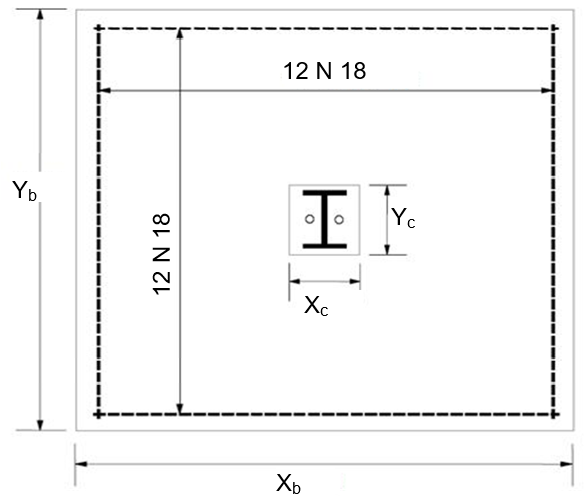
\includegraphics[width=10.72cm, height=8.94cm]{Figure3.png}\\
\centering
Figure 3. Plan view of the footing for a single column (not to scale), with steel reinforcements 12$\times$N18 (diameter 18 mm) in each direction\\
\centering
\end{figure}
\\
\\
\\
\begin{textblock*}{5cm}(8.9cm,28.49cm)
Page
\end{textblock*}
\begin{textblock*}{5cm}(10.1cm,28.49cm)
of 5
\end{textblock*}
\newpage
\noindent
\textbf{QUESTION 5 [45 marks]}\\
A steel beam with the section of 250UB37.3 (in reference to BHP-300PLUS) is simply supported by two columns of 250UC72.9 (in reference to BHP-300PLUS) as shown in Figure 4. The length of the beam (L\textsubscript{b}) is $\py{sv51}$ m, whereas the length of the columns (L\textsubscript{c}) is $\py{sv52}$ m. A secondary beam is placed on top of the beam at mid-span applying a concentrated load P at the top flange of the beam, as shown in Figure 4.\\
\\
f\textsubscript{y} = $\py{sv53}$ MPa\\
E = Young’s modulus of elasticity = 200,000 MPa.\\
G = shear modulus of elasticity = 80,000 MPa.\\
Capacity factor \phi = 0.9\\
$\alpha_b$ = 0, $k_f$ = 1\\
\\
a) The beam is simple supported at both ends (assuming full restraint without lateral rotation restraint) and the secondary beam effectively restrain the lateral deflection at mid-span. Calculate the maximum value of P the beam can resist assuming the out-of-plane buckling is not prevented. The bending moment diagram of the beam is reported in Figure 4. \textbf{[12 marks]}\\
\\
b) Assume now that the maximum bending moment of the beam at mid-span is equal to $\py{sv54}$ kNm and that an axial force N* in compression is also applied to the beam, what is the maximum value of N* the member can resist if the general equation is used? Assume that the out-of-plane buckling of the member is not prevented. The effective length factor k\textsubscript{e} is taken as $\py{sv55}$ in determining the column capacity in compression alone. \textbf{[12 marks]}\\
\\
c) Assume that under certain loading combinations, the bending moment diagram for the columns is a straight line with the maximum moment M\textsubscript{x}* of $\py{sv56}$ kNm at the base of the column (refer to the bending moment diagram in Figure 4). The boundary conditions for the column can be assumed as FF without rotational restraints. Assume the out-of-plane buckling of the column is not prevented and its effective length factor k\textsubscript{e} is $\py{sv57}$, what is the maximum allowed axial force N* in the column if the formula for special I-section is adopted?  \textbf{[12 marks]}\\
\\
d) Consider now the column under the same bending moment (straight line with the maximum moment M\textsubscript{x}* of $\py{sv56}$ kNm at the base of the column) and a compression force equal to 200 kN. Calculate the amplified bending moment of the column by considering second order effects. Assume that the effective length factor k\textsubscript{e} is $\py{sv57}$. \textbf{[9 marks]}\\
\begin{figure}[ht]
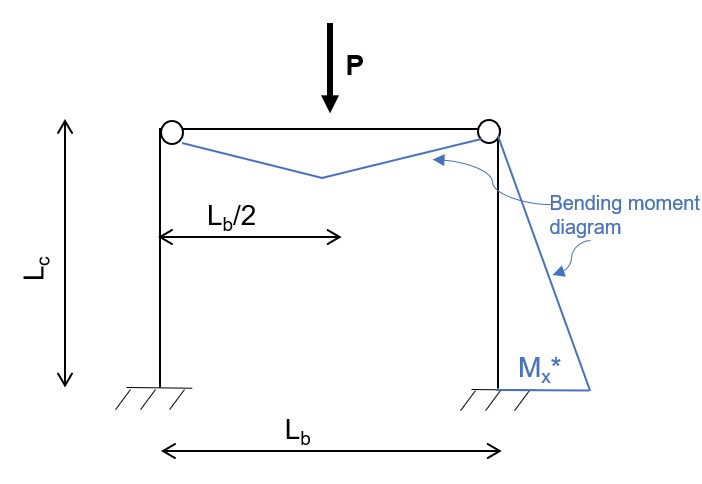
\includegraphics[width=10.64cm, height=7.33cm]{Figure4.png}\\
\centering
Figure 4\\
\centering
\end{figure}
\\
\begin{textblock*}{5cm}(8.9cm,28.49cm)
Page
\end{textblock*}
\begin{textblock*}{5cm}(10.1cm,28.49cm)
of 5
\end{textblock*}
\begin{hidden}	
\clearpage
\section{Solution}

\textbf{Step 1:} Define coordinate system. This is already provided in \Cref{fig:grid}. 

\textbf{Step 2:} The unknown degrees of freedom are: 

\begin{itemize}
	\item Rotation about global y-axis at C ($\theta_C$)
	\item Rotation about global y-axis at D ($\theta_D$)
	\item Rotation about global y-axis at F ($\theta_F$)
\end{itemize} 

Due to symmetry of members CD and CF, and no applied point load, the degree of freedom for translation C is known: $\delta_C = 0$. Hence; 

\begin{equation}
	DOF = \left\{\theta_C,\theta_D,\theta_F\right\}
\end{equation}

\textbf{Step 3:} The known forces corresponding to the unknown DOF are: 

\begin{equation}
	F = \left\{ \py{n(M)},0,0 \right\} \textrm{\hspace{0.5cm} [kNm]}
\end{equation}

Note, the negative sign as per the direction of the double-headed arrow. 
	
\textbf{Step 4:} Apply $\theta_C$ positively only. 

This causes bending along member DCF, and twisting along member ECG. 

\textbf{Step 5:} Get forces at each DOF. 

Moment in the direction of $\theta_C$ caused by $\theta_C$: 

\begin{itemize}
	\item In Element DC: $M_C = \left(\frac{4EI}{L}\right)\theta_C$
	\item In Element CF: $M_C = \left(\frac{4EI}{L}\right)\theta_C$
	\item In Element EC: $M_C = \left(\frac{GJ}{L}\right)\theta_C$
	\item In Element CG: $M_C = \left(\frac{GJ}{L}\right)\theta_C$
\end{itemize}	

As all member properties are equal, then: 

\begin{equation}
	M_C = \frac{8EI+2GJ}{L}\theta_C
\end{equation}

Moment in the direction of $\theta_D$ caused by $\theta_C$: 

\begin{itemize}
	\item In Element DC: $M_D = \left(\frac{2EI}{L}\right)\theta_C$
\end{itemize}	

Moment in the direction of $\theta_F$ caused by $\theta_C$: 

\begin{itemize}
	\item In Element CF: $M_F = \left(\frac{2EI}{L}\right)\theta_C$
\end{itemize}	

\textbf{Step 6:} Repeat for each DOF

Apply $\theta_D$ positively only and get forces at each DOF. 

Moment in the direction of $\theta_C$ caused by $\theta_D$: 

\begin{itemize}
	\item In Element DC: $M_C = \left(\frac{2EI}{L}\right)\theta_D$
\end{itemize}	

Moment in the direction of $\theta_D$ caused by $\theta_D$: 

\begin{itemize}
	\item In Element DC: $M_D = \left(\frac{4EI}{L}\right)\theta_D$
\end{itemize}	

Moment in the direction of $\theta_F$ caused by $\theta_D$ is equal to zero ($M_F = 0$) as there is no rotation (C is locked).

Apply $\theta_F$ positively only and get forces at each DOF. 

Moment in the direction of $\theta_C$ caused by $\theta_F$: 

\begin{itemize}
	\item In Element DC: $M_C = \left(\frac{2EI}{L}\right)\theta_F$
\end{itemize}	

Moment in the direction of $\theta_D$ caused by $\theta_F$ is equal to zero ($M_D = 0$) as there is no rotation (C is locked).		

Moment in the direction of $\theta_F$ caused by $\theta_F$: 

\begin{itemize}
	\item In Element DC: $M_F = \left(\frac{4EI}{L}\right)\theta_F$
\end{itemize}			
		
\textbf{Step 7:} Add nodal forces

Total moment in the direction of $\theta_C$: 

\begin{equation}
	M_C = \frac{8EI+2GJ}{L}\theta_C +  \left(\frac{2EI}{L}\right)\theta_D + \left(\frac{2EI}{L}\right)\theta_F  
\end{equation}

Total moment in the direction of $\theta_D$: 

\begin{equation}
	M_D = \left(\frac{2EI}{L}\right)\theta_C + \left(\frac{4EI}{L}\right)\theta_D + 0  
\end{equation}

Total moment in the direction of $\theta_F$:

\begin{equation}
	M_F = \left(\frac{2EI}{L}\right)\theta_C + 0 \left(\frac{4EI}{L}\right)\theta_F  
\end{equation}

Given: 

\begin{equation}
\frac{EI}{L} = \frac{ \left( \py{to_eng(E)} \right)\left(\py{to_eng(I)}\right) }
					{ \left(\py{to_eng(L)}\right) } \times 10^{-3}
				=\py{to_eng(EI_L*1e3)}~\mathrm{kNm}
\end{equation}


\begin{equation}
\frac{GJ}{L} = \frac{ \left( \py{to_eng(G)} \right)\left(\py{to_eng(J)}\right) }
					{ \left(\py{to_eng(L)}\right) } \times 10^{-3}
				=\py{to_eng(GJ_L*1e3)}~\mathrm{kNm}
\end{equation}

The resulting structural stiffness matrix becomes: 

\begin{equation}
	K = 10^3 \py{m2ltx(sysK(grid))}
\end{equation}

Notice, it is symmetrical, giving confidence we have done it correctly.  

\textbf{Step 8:} Solve, using Rule of Sarrus and Cramer's Rule to find:
	
\begin{align*}
	\begin{Bmatrix}
		\theta_C \\ \theta_D \\ \theta_F
	\end{Bmatrix} 
	&= 10^{-3} 
	{\py{m2ltx(sysK(grid))}}^{-1}
	\py{m2ltx(getF(grid),style='Bmatrix')} \\
	&= \frac{10^{-3}}{\py{to_eng(det_K(sysK(grid)))}} \py{m2ltx(inv_K(sysK(grid))*det_K(sysK(grid)))}
	\py{m2ltx(getF(grid),style='Bmatrix')} \\
\end{align*}
from which:
\begin{equation}
	\begin{Bmatrix}
		\theta_C \\ \theta_D \\ \theta_F
	\end{Bmatrix} 
	= \py{m2ltx(D*1e3,style='Bmatrix')}	~\mathrm{[mrad]}
\end{equation}

\textbf{Step 9:} Member forces:

Using the special matrix since there is no vertical force and no
vertical displacement for this special case.

For Member \emph{CD}:
\begin{equation*}
	\begin{Bmatrix}
	T_C \\ M_C \\ T_D \\ M_D
	\end{Bmatrix} 
	= 10^{3} 
	\py{m2ltx(eleK(grid))}
	\py{m2ltx(d_CD(D*1e3),style='Bmatrix')}
	= 
	\py{m2ltx(Fcd,style='Bmatrix')}
	~\mathrm{[kNm]}
\end{equation*}

For Member \emph{CF} we consider not using the lower number node as the $i$ node to illustrate the coordinate transform that must be considered. In this case, since the local $z$-axis and gloabl $Y$-axis are parallel, positive $\theta$ become positive major axis bending in the member's local coordinate system:

\begin{equation*}
	\begin{Bmatrix}
		T_C \\ M_C \\ T_F \\ M_F
	\end{Bmatrix} 
	= 10^{3} 
	\py{m2ltx(eleK(grid))}
	\py{m2ltx(d_FC(D*1e3),style='Bmatrix')}
	= 
	\py{m2ltx(Fcf,style='Bmatrix')}
	~\mathrm{[kNm]}
\end{equation*}


For Member \emph{CE}:
\begin{equation*}
	\begin{Bmatrix}
		T_C \\ M_C \\ T_E \\ M_E
	\end{Bmatrix} 
	= 10^{3} 
	\py{m2ltx(eleK(grid))}
	\py{m2ltx(d_CE(D*1e3),style='Bmatrix')}
	= 
	\py{m2ltx(Fce,style='Bmatrix')}
	~\mathrm{[kNm]}
\end{equation*}

And finally, for Member \emph{CG}, we again break convention and carefully consider the directions of the global displacements as they relate to the local member coordinate system.

\begin{equation*}
	\begin{Bmatrix}
		T_G \\ M_G \\ T_C \\ M_C
	\end{Bmatrix} 
	= 10^{3} 
	\py{m2ltx(eleK(grid))}
	\py{m2ltx(d_GC(D*1e3),style='Bmatrix')}
	= 
	\py{m2ltx(Fgc,style='Bmatrix')}
	~\mathrm{[kNm]}
\end{equation*}

\textbf{Step 10} is to draw the internal actions diagrams. To do this, the results of the member actions which were derived in the local member coordinate system must now be considered now in the global coordinate system. The easiest way to do this is to draw the directions by carefully interpreting the member force signs against the global axis system. The resulting FBD is shown in \Cref{fig:fbd}.

\begin{figure}[!htb]
	\centering
	
	\begin{pysub}
		\setcoords{-25}{30}[1][1] 
		\setaxis{2} 
		\begin{adjustbox}{max width=\textwidth}
			\begin{tikzpicture}[coords] 
			\dscaling{1}{1.5};
			
			\dpoint{c}{0}{0}{0}; 
			\dpoint{d}{ -!{L} }{0}{0};
			\dpoint{e}{0}{ !{L} }{0}; 
			\dpoint{f}{ !{L} }{0}{0};
			\dpoint{g}{0}{-!{L} }{0}; 
			\dpoint{z}{ -!{0.7*L} }{ -!{0.7*L} }{0}; 
			
			\daxis{1}{z}; 
			
			\dbeam{1}{c}{d};
			\dbeam{1}{c}{e};
			\dbeam{1}{c}{f};
			\dbeam{1}{c}{g};
			
			\support{1}{d}; \hinge{1}{d}
			\support{3}{e}[90];
			\support{1}{f}; \hinge{1}{f}
			\support{3}{g}[270];

			\begin{scope}[force/.append style={color=red,>={Latex[length=0pt 5]}},
			normalLine/.append style={line width=1mm}]
				
				\dload{4}{c}[90][-90][ !{L/3} ];
				\dnotation{1}{c}{$!{n(abs(Fcg[0]))}$}[left=5mm];

				\dload{3}{c}[270][-90][ !{L/3} ];
				\dnotation{1}{c}{$!{n(abs(Fce[0]))}$}[right=5mm];				
				
				\dpoint{cd}{-!{L/6}}{0}{0}
				\dload{4}{cd}[90][-90][ !{L/3} ];
				\dnotation{1}{cd}{$!{n(abs(Fcd[1]))}$}[left=5mm];

				\dpoint{cf}{!{L/6}}{0}{0}
				\dload{4}{cf}[90][-90][ !{L/3} ];
				\dnotation{1}{cf}{$!{n(abs(Fcf[1]))}$}[below=5mm];
				
				\dload{4}{g}[270][-90][ !{L/3} ];
				\dnotation{1}{g}{$!{n(abs(Fcg[2]))}$}[right=5mm];

				\dload{3}{e}[90][-90][ !{L/3} ];
				\dnotation{1}{e}{$!{n(abs(Fce[2]))}$}[left=5mm];	
				
			\end{scope}
			
			\dnotation{1}{c}{$C$}[above=2mm];
			\dnotation{1}{d}{$D$}[above right];
			\dnotation{1}{e}{$E$}[above left];
			\dnotation{1}{f}{$F$}[above right];
			\dnotation{1}{g}{$G$}[below right];
			
			\end{tikzpicture}
		\end{adjustbox}
	\end{pysub}
	\caption{Free body diagram.}
	\label{fig:fbd}
\end{figure}

Considering the BMD, for each member, to identify the side in tension it can help to visualise the deformation resulting from the forces acting on it indicated in the free body diagram, \Cref{fig:fbd}. Since there are no loads acting between the nodes, the BMD is comprised of straight lines between the values at each node. The BMD is shown in \Cref{fig:bmd}.

\begin{figure}[ht]
	\centering
	
	\begin{pysub}
		\setcoords{-25}{30}[1][1][1] 
		\setaxis{2} 
		\begin{adjustbox}{max width=\textwidth}
			\begin{tikzpicture}[coords] 
			\dscaling{1}{1.5};
			
			\dpoint{c}{0}{0}{0}; 
			\dpoint{d}{ -!{L} }{0}{0};
			\dpoint{e}{0}{ !{L} }{0}; 
			\dpoint{f}{ !{L} }{0}{0};
			\dpoint{g}{0}{-!{L} }{0}; 
			\dpoint{z}{ -!{0.7*L} }{ -!{0.7*L} }{0}; 
			
			\daxis{1}{z}; 
			
			\dbeam{1}{c}{d};
			\dbeam{1}{c}{e};
			\dbeam{1}{c}{f};
			\dbeam{1}{c}{g};
			
			\support{1}{d};  \hinge{1}{d}
			\support{3}{e}[90];
			\support{1}{f};  \hinge{1}{f}
			\support{3}{g}[270];
			
			\dinternalforces{xz}{c}{d}{ !{int(Fcd[1]/bmd_scale)} }{ !{int(Fcd[3]/bmd_scale)} };
			\dinternalforces{xz}{c}{e}{ !{int(Fce[1]/bmd_scale)} }{ !{int(Fce[3]/bmd_scale)} };
			\dinternalforces{xz}{c}{f}{ !{int(Fcf[1]/bmd_scale)} }{ !{int(Fcf[3]/bmd_scale)} };
			\dinternalforces{xz}{c}{g}{ !{int(Fcg[1]/bmd_scale)} }{ !{int(Fcg[3]/bmd_scale)} };
			
			\dnotation{1}{c}{$!{n(abs(Fcd[1]))}$}[below right=18mm and 0mm of c];
			\dnotation{1}{c}{$!{n(abs(Fcf[1]))}$}[above left=18mm and 0mm of c];
			
			\dnotation{1}{c}{$C$}[right=3mm];
			\dnotation{1}{d}{$D$}[above right];
			\dnotation{1}{e}{$E$}[above left];
			\dnotation{1}{f}{$F$}[above right];
			\dnotation{1}{g}{$G$}[below right];
			
			\end{tikzpicture}
		\end{adjustbox}
	\end{pysub}
	\caption{Bending Moment Diagram.}
	\label{fig:bmd}
\end{figure}

For the TMD, it is not necessary to adopt a strict drawing convention once the relative actions are indicated. For example, the double-headed arrow in \Cref{fig:fbd} indicating the torsion of member $CE$ could be thought of as an analogous ``tension'' which we may consider as positive, and so we draw the TMD above the line. Similarly, fr member $CG$, the double-headed arrows act in the opposite sense to the analogous ``tension'' and so are analogous to ``compression'', which we then draw on the bottom of the member, as shown in \Cref{fig:tmd}.

\begin{figure}[ht]
	\centering
	
	\begin{pysub}
		\setcoords{-25}{30}[1][1][1] 
		\setaxis{2} 
		\begin{adjustbox}{max width=\textwidth}
			\begin{tikzpicture}[coords] 
			\dscaling{1}{1.5};
			
			\dpoint{c}{0}{0}{0}; 
			\dpoint{d}{ -!{L} }{0}{0};
			\dpoint{e}{0}{ !{L} }{0}; 
			\dpoint{f}{ !{L} }{0}{0};
			\dpoint{g}{0}{-!{L} }{0}; 
			\dpoint{z}{ -!{0.7*L} }{ -!{0.7*L} }{0}; 
			
			\daxis{1}{z}; 
			
			\dbeam{1}{c}{d};
			\dbeam{1}{c}{e};
			\dbeam{1}{c}{f};
			\dbeam{1}{c}{g};
			
			\support{1}{d};  \hinge{1}{d}
			\support{3}{e}[90];
			\support{1}{f};  \hinge{1}{f}
			\support{3}{g}[270];
			
			\dinternalforces{yz}{c}{d}{ !{int(Fcd[0]/tmd_scale)} }{ !{int(-Fcd[2]/tmd_scale)} };
			\dinternalforces{yz}{c}{e}{ !{int(Fce[0]/tmd_scale)} }{ !{int(-Fce[2]/tmd_scale)} };
			\dinternalforces{yz}{c}{f}{ !{int(Fcf[0]/tmd_scale)} }{ !{int(-Fcf[2]/tmd_scale)} };
			\dinternalforces{yz}{c}{g}{ !{int(Fcg[0]/tmd_scale)} }{ !{int(-Fcg[2]/tmd_scale)} };
			
			\dnotation{1}{c}{$!{n(abs(Fce[0]))}$}[below=12mm];
			\dnotation{1}{e}{$!{n(abs(Fce[2]))}$}[above=12mm];
			\dnotation{1}{c}{$!{n(abs(Fcg[0]))}$}[above=12mm];
			\dnotation{1}{g}{$!{n(abs(Fcg[2]))}$}[below=12mm];
			
			\dnotation{1}{c}{$C$}[right=3mm];
			\dnotation{1}{d}{$D$}[above right];
			\dnotation{1}{e}{$E$}[above left];
			\dnotation{1}{f}{$F$}[above right];
			\dnotation{1}{g}{$G$}[below right];
			
			\end{tikzpicture}
		\end{adjustbox}
	\end{pysub}
	\caption{Torsion Moment Diagram.}
	\label{fig:tmd}
\end{figure}

\end{hidden}
\end{document}
